在上一章中我们了解到，深度神经网络通常比浅层神经网络更难训练. 这很不幸，因为我们有充分的理由相信，\emph{如果}我们能训练深度网络，它们会比浅层网络强大得多. 但是，尽管上一章传来的消息令人沮丧，我们不会让它阻止我们. 在本章中，我们将开发可用于训练深度网络的技术，并将它们付诸实践. 我们还将审视更广阔的图景，简要回顾使用深度网络进行图像识别、语音识别和其他应用的最新进展. 并且我们将简要而带有推测性地展望神经网络和人工智能的未来.

本章篇幅较长. 为了帮助你导航，让我们先浏览一下. 各节之间耦合较松，因此只要你对神经网络有一些基本的了解，就可以跳到你最感兴趣的部分.

本章的主要部分是对最广泛使用的深度网络类型之一的介绍：深度卷积网络. 我们将通过一个详细的例子——包括代码在内的全部内容——来展示如何使用卷积网络解决从 MNIST 数据集中分类手写数字的问题：

\begin{center}
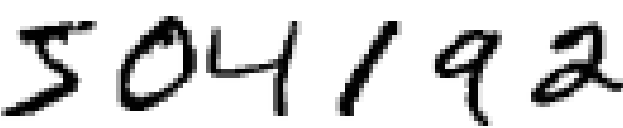
\includegraphics[width=0.267\textwidth]{images/digits.png}
\end{center}

\noindent 我们将从本书前面用于攻克这个问题的浅层网络开始讲述卷积网络. 通过多次迭代，我们将构建出越来越强大的网络. 在此过程中，我们将探索许多强大的技术：卷积、池化、使用 GPU 进行比浅层网络多得多的训练、训练数据的算法扩展（以减少过拟合）、dropout 技术的使用（同样是为了减少过拟合）、网络集成（ensemble）的使用，等等. 结果将是一个性能接近人类的系统. 在 10,000 张 MNIST 测试图像中——这些图像在训练期间从未见过！——我们的系统将正确分类 9,967 张. 下面是那 33 张被错误分类的图像的预览. 注意正确的分类在右上角；我们程序的分类在右下角：

\begin{center}
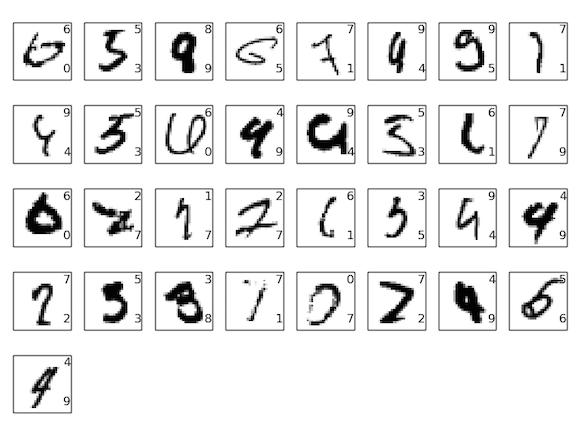
\includegraphics[width=0.967\textwidth]{images/ensemble_errors.png}
\end{center}

\noindent 其中许多图像即使对人类来说也很难分类. 例如，考虑第一行中的第三张图像. 在我看来它更像是一个 ``9'' 而不是官方分类的 ``8''. 我们的网络也认为它是一个 ``9''. 这种 ``错误'' 至少是可以理解的，甚至可能是值得称赞的. 我们以对使用网络（特别是卷积网络）进行图像识别的一些引人注目的最新进展的综述来结束关于图像识别的讨论.

本章的剩余部分从更广阔、更粗略的角度讨论深度学习. 我们将简要概述其他神经网络模型，例如循环神经网络和长短期记忆网络\label{term:68}，以及这些模型如何应用于语音识别、自然语言处理和其他领域的问题. 我们还将推测神经网络和深度学习的未来，从意图驱动的用户界面等想法，到深度学习在人工智能中的作用.

本章建立在本书前面章节的基础上，利用并整合了反向传播、正则化、softmax 函数等思想. 然而，要阅读本章，你不需要详细地学习过所有前面的章节. 不过，阅读第 1 章关于神经网络基础的内容会有所帮助. 当我使用第 2 章到第 5 章的概念时，我会提供链接，以便你在必要时熟悉它们.

值得注意的是本章不是什么. 它不是关于最新最伟大的神经网络库的教程. 我们也不会训练具有数十层的深度网络来解决最前沿的问题. 相反，重点是理解深度神经网络背后的一些核心原理，并将它们应用于 MNIST 问题这个简单、易于理解的背景中. 换句话说：本章不会把你直接带到前沿. 相反，本章和前面章节的目的是聚焦于基础，从而为你理解当前广泛的工作做好准备.
\sectionTitle{卷积网络入门}{卷积网络入门}

在前面的章节中，我们教会了神经网络相当出色地识别手写数字图像：

\begin{center}
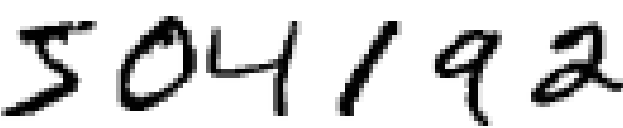
\includegraphics[width=0.267\textwidth]{images/digits.png}
\end{center}

\noindent 我们使用的网络中，相邻的网络层之间是全连接的. 也就是说，网络中的每一个神经元都与相邻层中的每一个神经元相连：

\begin{center}
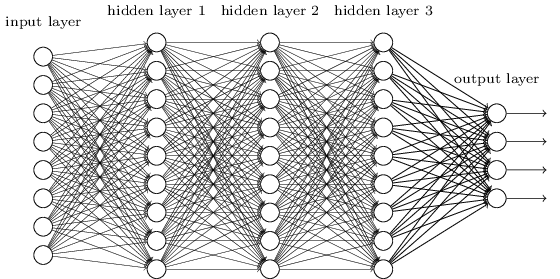
\includegraphics[width=0.9\textwidth]{images/tikz41.png}
\end{center}

\noindent 特别地，对于输入图像中的每个像素，我们将该像素的强度编码为输入层中对应神经元的值. 对于我们一直使用的 $28 \times 28$ 像素图像，这意味着我们的网络有 $784$（$= 28 \times 28$）个输入神经元. 然后我们训练网络的权重和偏置，使得网络的输出能够——我们希望如此！——正确地识别输入图像：'0'、'1'、'2'、...、'8' 或 '9'.

我们之前的网络工作得相当不错：使用 MNIST 手写数字数据集的训练和测试数据，我们获得了超过 98\% 的分类准确率. 但仔细想想，使用全连接层网络来分类图像是很奇怪的. 原因在于，这样的网络结构没有考虑图像的空间结构. 例如，它将相距很远和靠得很近的输入像素完全同等对待. 这种空间结构的概念必须从训练数据中推断出来. 但是，如果我们不是从一个\emph{白板}式的网络结构出发，而是使用一种试图利用空间结构的结构呢？在本节中，我将介绍\emph{卷积神经网络}*\footnote{卷积神经网络的起源可以追溯到 20 世纪 70 年代. 但奠定现代卷积网络这一学科的奠基性论文是 1998 年 Yann LeCun、Léon Bottou、Yoshua Bengio 和 Patrick Haffner 发表的 ``Gradient-based learning applied to document recognition''. LeCun 后来对卷积网络的术语发表了一个有趣的评论：``像卷积网络这样的模型中的[生物学]神经灵感是非常微弱的. 这就是为什么我称它们为'卷积网络'而不是'卷积神经网络'，也是为什么我们称节点为'单元'而不是'神经元' ''. 尽管有这番评论，卷积网络使用了与我们迄今为止所研究的神经网络许多相同的思想：诸如反向传播、梯度下降、正则化、非线性激活函数等等. 因此我们将遵循惯例，将它们视为一种神经网络. 我将交替使用术语``卷积神经网络''和``卷积网络''. 我也将交替使用术语``[人工]神经元''和``单元''.}. 这些网络使用一种特别适合分类图像的特殊结构. 使用这种结构使得卷积网络训练速度很快. 这反过来又帮助我们训练深层的多层网络，这些网络非常擅长分类图像. 如今，大多数用于图像识别的神经网络都使用深度卷积网络或某种接近的变体.

卷积神经网络\label{term:69}使用三个基本思想：\emph{局部感受野}、\emph{权重共享}和\emph{池化}. 让我们依次来看这些思想. \textbf{局部感受野：} 在前面展示的全连接层中，输入被描绘成一条垂直的神经元线. 在卷积网络中，将输入视为一个 $28 \times 28$ 的神经元方块会更有帮助，其值对应于我们用作输入的 $28 \times 28$ 像素强度：

\begin{center}
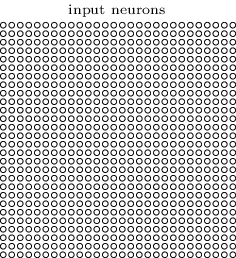
\includegraphics[width=0.9\textwidth]{images/tikz42.png}
\end{center}

\noindent 和往常一样，我们将输入像素连接到一层隐藏神经元. 但我们不会将每个输入像素连接到每个隐藏神经元. 相反，我们只在输入图像的小的局部区域内建立连接.

更准确地说，第一个隐藏层中的每个神经元将连接到输入神经元的一个小区域，比如说，一个 $5 \times 5$ 的区域，对应 $25$ 个输入像素. 因此，对于某个特定的隐藏神经元，我们可能有这样的连接：

\begin{center}
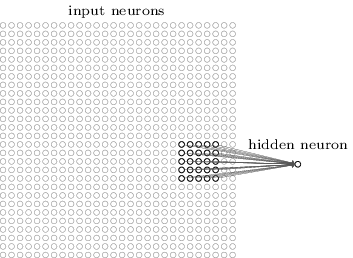
\includegraphics[width=0.9\textwidth]{images/tikz43.png}
\end{center}

\noindent 输入图像中的那个区域被称为该隐藏神经元的\emph{局部感受野}. 它是输入像素上的一个小窗口. 每个连接学习一个权重. 隐藏神经元还学习一个总的偏置. 你可以把那个特定的隐藏神经元看作是在学习分析它特定的局部感受野.

然后我们将局部感受野\label{term:70}在整个输入图像上滑动. 对于每个局部感受野，第一个隐藏层中都有一个不同的隐藏神经元. 为了具体说明这一点，让我们从左上角的一个局部感受野开始：

\begin{center}
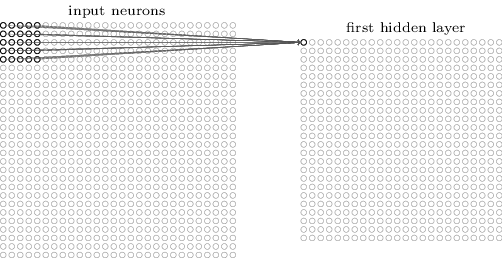
\includegraphics[width=0.9\textwidth]{images/tikz44.png}
\end{center}

\noindent 然后我们将局部感受野向右滑动一个像素（即一个神经元），连接到第二个隐藏神经元：

\begin{center}
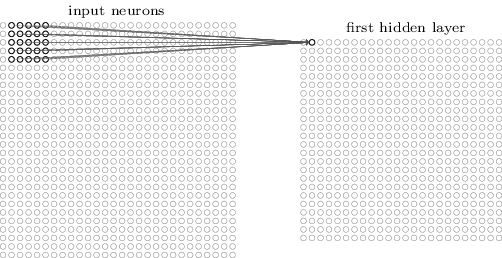
\includegraphics[width=0.9\textwidth]{images/tikz45.png}
\end{center}

\noindent 以此类推，构建出第一个隐藏层. 注意，如果我们有一个 $28 \times 28$ 的输入图像，以及 $5 \times 5$ 的局部感受野，那么隐藏层中将有 $24 \times 24$ 个神经元. 这是因为我们只能将局部感受野移动 $23$ 个神经元（或向下 $23$ 个神经元），否则就会碰到输入图像的右侧（或底部）.

我展示的是局部感受野每次移动一个像素. 事实上，有时会使用不同的\emph{步长}. 例如，我们可能将局部感受野向右（或向下）移动 $2$ 个像素，在这种情况下我们会说使用了步长 $2$. 在本章中，我们主要坚持使用步长 $1$，但值得知道的是，人们有时会尝试不同的步长*\footnote{正如前面章节所做的那样，如果我们有兴趣尝试不同的步长，那么我们可以使用验证数据来挑选出性能最佳的步长. 更多细节，请参见前面关于如何选择神经网络超参数的讨论. 同样的方法也可以用来选择局部感受野的大小——当然，使用 $5 \times 5$ 的局部感受野并没有什么特别之处. 一般来说，当输入图像明显大于 $28 \times 28$ 像素的 MNIST 图像时，更大的局部感受野往往更有帮助.}. \textbf{权重共享\label{term:71}和偏置共享：} 我说过每个隐藏神经元都有一个偏置和连接到其局部感受野的 $5 \times 5$ 个权重. 我还没有提到的是，我们将对 $24 \times 24$ 个隐藏神经元中的每一个使用\emph{相同}的权重和偏置. 换句话说，对于第 $j, k$ 个隐藏神经元，输出为：

\begin{equation}
\sigma\left(b + \sum_{l=0}^4 \sum_{m=0}^4 w_{l,m} a_{j+l, k+m} \right).
\tag{125}
\end{equation}

\noindent 这里，$\sigma$ 是神经激活函数——也许是我们在前面章节中使用的 S 型函数. $b$ 是偏置的共享值. $w_{l,m}$ 是一个 $5 \times 5$ 的共享权重数组. 最后，我们用 $a_{x, y}$ 表示位置 $x, y$ 处的输入激活值.

这意味着第一个隐藏层中的所有神经元检测完全相同的特征*\footnote{我还没有精确定义特征的概念. 非正式地说，把隐藏神经元检测到的特征看作是将导致该神经元激活的那类输入模式：例如，它可能是图像中的一条边缘，或者也许是某种其他类型的形状.}，只是在输入图像中的不同位置. 要理解为什么这是合理的，假设权重和偏置使得隐藏神经元能够挑出，比如说，某个特定局部感受野中的一条垂直边缘. 这种能力在图像的其他地方也很可能有用. 因此，在图像的每个地方应用相同的特征检测器是有用的. 用稍微更抽象的话来说，卷积网络很好地适应了图像的平移不变性：将一张猫的图片（比如说）移动一点，它仍然是一张猫的图片*\footnote{事实上，对于我们一直在研究的 MNIST 数字分类问题，图像是居中的且大小归一化的. 所以可以说，MNIST 比``在野外''发现的图像具有更少的平移不变性. 尽管如此，像边缘和角这样的特征在输入空间的大部分区域很可能是有用的.}.

出于这个原因，我们有时将输入层到隐藏层的映射称为\emph{特征图}. 我们将定义特征图的权重称为\emph{共享权重}. 我们将以这种方式定义特征图的偏置称为\emph{共享偏置}. 共享权重和偏置通常被说成定义了一个\emph{核}或\emph{滤波器}. 在文献中，人们有时以略微不同的方式使用这些术语，因此我不会更精确地定义；相反，稍后我们将看一些具体的例子.

到目前为止我描述的网络结构只能检测一种局部特征. 要进行图像识别，我们需要不止一个特征图\label{term:73}. 因此，一个完整的卷积层\label{term:72}由几个不同的特征图组成：

\begin{center}
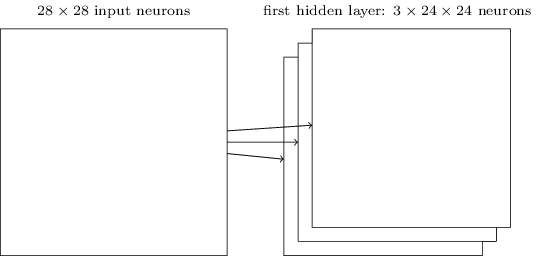
\includegraphics[width=0.9\textwidth]{images/tikz46.png}
\end{center}

\noindent 在所示的例子中，有 $3$ 个特征图. 每个特征图由一组 $5 \times 5$ 的共享权重和一个共享偏置定义. 结果是网络可以检测 $3$ 种不同的特征，每种特征都可以在整个图像中被检测到.

我只展示了 $3$ 个特征图，以使上面的图保持简单. 然而，在实践中，卷积网络可能使用更多（也许多得多）的特征图. 早期的卷积网络之一，LeNet-5，使用了 $6$ 个特征图，每个关联到一个 $5 \times 5$ 的局部感受野，来识别 MNIST 数字. 所以上面展示的例子实际上非常接近 LeNet-5. 在本章后面我们开发的例子中，我们将使用具有 $20$ 和 $40$ 个特征图的卷积层. 让我们快速看一下学习到的一些特征*\footnote{所展示的特征图来自我们训练的最终卷积网络，见这里.}：

\begin{center}
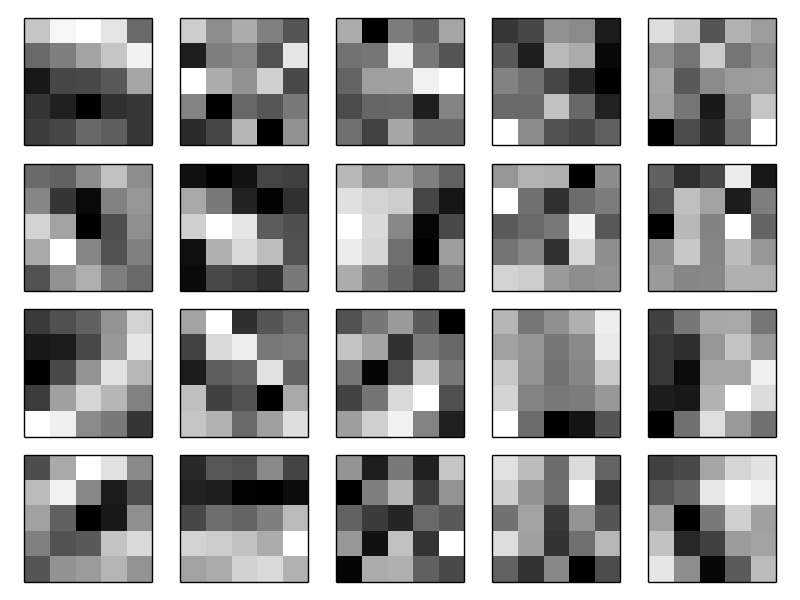
\includegraphics[width=0.667\textwidth]{images/net_full_layer_0.png}
\end{center}

\noindent 这 $20$ 张图像对应于 $20$ 个不同的特征图（或滤波器，或核）. 每个图表示为一个 $5 \times 5$ 的块图像，对应于局部感受野中的 $5 \times 5$ 个权重. 较白的块意味着较小的（通常更负的）权重，因此特征图对相应的输入像素响应较弱. 较暗的块意味着较大的权重，因此特征图对相应的输入像素响应较强. 非常粗略地说，上面的图像显示了卷积层所响应的特征类型.

那么我们能从这些特征图中得出什么结论呢？很明显，这里存在超出我们随机预期的空间结构：许多特征具有明显的亮暗子区域. 这表明我们的网络确实在学习与空间结构相关的东西. 然而，除此之外，很难看出这些特征检测器在学习什么. 当然，我们不是在学习（比如说）许多传统图像识别方法中使用的 Gabor 滤波器. 事实上，现在有大量工作致力于更好地理解卷积网络学习到的特征. 如果你有兴趣跟进这项工作，我建议从 Matthew Zeiler 和 Rob Fergus（2013）的论文 Visualizing and Understanding Convolutional Networks 开始.

共享权重和偏置的一大优势是它大大减少了卷积网络中涉及的参数数量. 对于每个特征图，我们需要 $25 = 5 \times 5$ 个共享权重，加上一个共享偏置. 所以每个特征图需要 $26$ 个参数. 如果我们有 $20$ 个特征图，那就是总共 $20 \times 26 = 520$ 个参数来定义卷积层. 相比之下，假设我们有一个全连接的第一层，有 $784 = 28 \times 28$ 个输入神经元，以及相对适中的 $30$ 个隐藏神经元，正如我们在本书前面许多例子中使用的那样. 那就是总共 $784 \times 30$ 个权重，加上额外的 $30$ 个偏置，总共 $23,550$ 个参数. 换句话说，全连接层的参数数量将是卷积层的 $40$ 倍以上.

当然，我们无法真正直接比较参数数量，因为这两个模型在本质上是不同的. 但是，直观上，卷积层利用平移不变性似乎很可能减少它达到与全连接模型相同性能所需的参数数量. 这反过来将导致卷积模型训练更快，并最终帮助我们使用卷积层构建深度网络.

顺便提一下，\emph{卷积}这个名字来源于方程 (125) 中的运算

\begin{align*}
\sigma\left(b + \sum_{l=0}^4 \sum_{m=0}^4 w_{l,m} a_{j+l, k+m} \right) \nonumber
\end{align*}
\noindent 有时被称为\emph{卷积}. 更准确地说，人们有时将该方程写为 $a^1 = \sigma(b + w * a^0)$，其中 $a^1$ 表示来自一个特征图的输出激活值集合，$a^0$ 是输入激活值集合，而 $*$ 被称为卷积运算. 我们不打算深入使用卷积的数学，所以你不需要太担心这个联系. 但至少值得知道这个名字从何而来.\textbf{池化层\label{term:74}：} 除了刚才描述的卷积层之外，卷积神经网络还包含\emph{池化层}. 池化层通常紧跟在卷积层之后使用. 池化层所做的是简化卷积层输出中的信息.

具体来说，池化层取卷积层输出的每个特征图*\footnote{这里的命名比较宽松. 特别地，我用``特征图''指的不是卷积层计算的函数，而是该层输出的隐藏神经元的激活值. 这种对命名的轻微滥用在研究文献中相当常见.}并准备一个浓缩的特征图. 例如，池化层中的每个单元可以汇总前一层中（比如）$2 \times 2$ 个神经元的区域. 作为一个具体例子，一种常见的池化过程被称为\emph{最大池化}. 在最大池化中，池化单元简单地输出 $2 \times 2$ 输入区域中的最大激活值，如下图所示：

\begin{center}
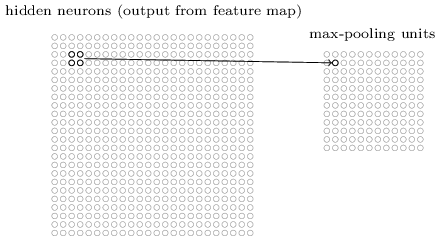
\includegraphics[width=0.9\textwidth]{images/tikz47.png}
\end{center}

\noindent 注意，由于卷积层输出 $24 \times 24$ 个神经元，池化后我们有 $12 \times 12$ 个神经元.

如上所述，卷积层通常涉及不止一个特征图. 我们对每个特征图分别应用最大池化\label{term:75}. 所以如果有三个特征图，组合的卷积层和最大池化层将如下所示：

\begin{center}
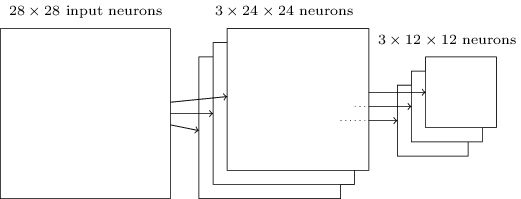
\includegraphics[width=0.9\textwidth]{images/tikz48.png}
\end{center}

\noindent 我们可以将最大池化视为网络询问给定特征是否在图像的某个区域中任何地方被找到的一种方式. 然后它丢弃精确的位置信息. 直觉是，一旦找到了一个特征，它的精确位置就不如它相对于其他特征的粗略位置那么重要. 一个很大的好处是池化后的特征少得多，因此这有助于减少后续层中所需的参数数量.

最大池化并不是用于池化的唯一技术. 另一种常见方法被称为\emph{L2 池化}. 在这里，我们不是取 $2 \times 2$ 神经元区域的最大激活值，而是取 $2 \times 2$ 区域中激活值平方和的平方根. 虽然细节不同，但直觉与最大池化相似：L2 池化是一种浓缩卷积层信息的方式. 在实践中，这两种技术都被广泛使用. 有时人们使用其他类型的池化操作. 如果你真的想优化性能，你可以使用验证数据来比较几种不同的池化方法，并选择效果最好的方法. 但我们不打算担心那种详细的优化.\textbf{整合所有内容：} 我们现在可以将所有这些想法整合在一起，形成一个完整的卷积神经网络. 它类似于我们刚才看到的架构，但增加了一层 $10$ 个输出神经元，对应于 MNIST 数字的 $10$ 个可能值（'0'、'1'、'2'、\emph{等等}）：

\begin{center}
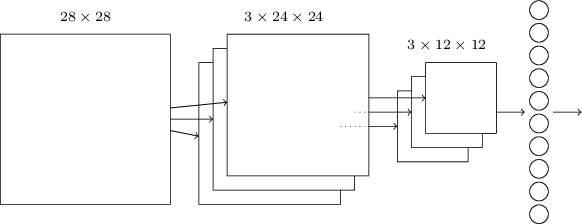
\includegraphics[width=0.9\textwidth]{images/tikz49.png}
\end{center}

\noindent 网络以 $28 \times 28$ 个输入神经元开始，用于编码 MNIST 图像的像素强度. 然后是一个使用 $5 \times 5$ 局部感受野和 $3$ 个特征图的卷积层. 结果是一层 $3 \times 24 \times 24$ 个隐藏特征神经元. 下一步是一个最大池化层，应用于 $2 \times 2$ 区域，跨越 $3$ 个特征图中的每一个. 结果是一层 $3 \times 12 \times 12$ 个隐藏特征神经元.

网络中最后一层连接是全连接层. 也就是说，这一层将最大池化层中的\emph{每一个}神经元连接到 $10$ 个输出神经元中的每一个. 这种全连接架构与我们前几章使用的相同. 但请注意，在上图中，为了简单起见，我使用了一个箭头，而不是显示所有连接. 当然，你可以很容易地想象这些连接.

这种卷积架构与前几章使用的架构相当不同. 但整体图景\label{term:76}是相似的：一个由许多简单单元组成的网络，其行为由它们的权重和偏置决定. 总体目标仍然相同：使用训练数据来训练网络的权重和偏置，以便网络能够很好地分类输入数字.

特别地，正如本书前面一样，我们将使用随机梯度下降和反向传播来训练我们的网络. 这基本上与前几章的方式完全相同. 然而，我们确实需要对反向传播过程做一些修改. 原因是我们之前对反向传播的推导是针对具有全连接层的网络. 幸运的是，修改卷积层和最大池化层的推导是直接的. 如果你想了解细节，那么我邀请你完成以下习题. 请注意，除非你已经真正内化了之前对反向传播的推导（在这种情况下它很容易），否则这个习题需要一些时间来完成.

\begin{exerciseBox}{习题}

\begin{itemize}

\item
\textbf{卷积网络中的反向传播} 具有全连接层的网络中反向传播的核心方程是 (BP1)

\begin{align*}
\delta^L_j = \frac{\partial C}{\partial a^L_j} \sigma'(z^L_j) \nonumber
\end{align*}

-(BP4)

\begin{align*}
\frac{\partial C}{\partial w^l_{jk}} = a^{l-1}_k \delta^l_j \nonumber
\end{align*}

(链接). 假设我们有一个包含卷积层、最大池化层和全连接输出层的网络，如上面讨论的网络. 反向传播的方程如何修改？

\end{itemize}

\end{exerciseBox}
\sectionTitle{卷积神经网络的实践}{卷积神经网络的实践}

我们已经看到了卷积神经网络背后的核心思想. 让我们通过实现一些卷积网络，并将它们应用于 MNIST 数字分类问题，来看看它们在实践中是如何工作的. 我们将用来完成这项工作的程序叫做 \texttt{network3.py}，它是前面几章中开发的程序 \texttt{network.py} 和 \texttt{network2.py} 的改进版本*\footnote{还要注意， \texttt{network3.py} 融合了 Theano 库关于卷积神经网络的文档中的思想（特别是 LeNet-5 的实现），来自 Misha Denil 的 dropout 实现，以及来自 Chris Olah 的思想.}. 如果你想跟着做，代码可以在 GitHub 上找到. 注意我们将在下一节中详细讨论 \texttt{network3.py} 本身的代码. 在本节中，我们将把 \texttt{network3.py} 作为一个库来构建卷积网络.

程序 \texttt{network.py} 和 \texttt{network2.py} 是用 Python 和矩阵库 Numpy 实现的. 那些程序从基本原理出发，深入到了反向传播、随机梯度下降等等的细节. 但既然我们已经理解了那些细节，对于 \texttt{network3.py}，我们将使用一个叫做 Theano 的机器学习库*\footnote{参见 Theano: A CPU and GPU Math Expression Compiler in Python，作者为 James Bergstra, Olivier Breuleux, Frederic Bastien, Pascal Lamblin, Ravzan Pascanu, Guillaume Desjardins, Joseph Turian, David Warde-Farley，和 Yoshua Bengio (2010). Theano 也是流行的 Pylearn2 和 Keras 神经网络库的基础. 在撰写本文时，其他流行的神经网络库包括 Caffe 和 Torch.}. 使用 Theano 使得为卷积神经网络实现反向传播变得容易，因为它自动计算所有涉及的映射. Theano 也比我们之前的代码快得多（之前的代码是为了易于理解而编写的，而不是为了快），这使得训练更复杂的网络变得实际可行. 特别是， Theano 的一个很棒的特性是它可以在 CPU 上运行代码，或者如果有的话，在 GPU 上运行. 在 GPU 上运行提供了显著的加速，并且再次帮助使训练更复杂的网络变得实际可行.

如果你想跟着做，那么你需要让你的系统上运行 Theano. 要安装 Theano，请按照项目主页上的说明进行操作. 下面这些例子是使用 Theano 0.6 运行的*\footnote{在我发布本章时， Theano 的当前版本已经变为 0.7 版. 我实际上在 Theano 0.7 下重新运行了这些例子，得到的结果与文中报告的极其相似.}. 有些是在 Mac OS X Yosemite 下运行的，没有 GPU. 有些是在 Ubuntu 14.04 下运行的，配有 NVIDIA GPU. 还有一些实验是在两种环境下都运行过的. 要让 \texttt{network3.py} 运行起来，你需要在 \texttt{network3.py} 源代码中将 \texttt{GPU} 标志设置为 \texttt{True} 或 \texttt{False}（视情况而定）. 除此之外，要让 Theano 在 GPU 上运行起来，你可能会发现这里的说明很有帮助. 网上也有教程，用 Google 很容易找到，可以帮助你让一切正常工作. 如果你本地没有可用的 GPU，那么你可能想了解一下 Amazon Web Services EC2 G2 竞价实例. 注意即使有 GPU，代码也需要一些时间来执行. 许多实验需要几分钟到几小时才能运行完. 在 CPU 上，最复杂的实验可能需要几天才能运行完. 和前面几章一样，我建议把程序跑起来，然后继续阅读，偶尔回来查看代码的输出. 如果你使用的是 CPU，你可能希望减少更复杂实验的训练轮次，或者干脆完全省略它们.

为了获得一个基线，我们将从一个浅层架构开始，只使用一个隐藏层，包含 $100$ 个隐藏神经元. 我们将训练 $60$ 个轮次，使用学习率 $\eta = 0.1$，小批量大小为 $10$，不使用正则化. 我们开始吧*\footnote{本节实验的代码可以在这个脚本中找到. 注意脚本中的代码只是重复和对应了本节的讨论.\\ \\ 还要注意，在整节中我都明确指定了训练轮次的数量. 我这样做是为了清楚地说明我们是如何训练的. 在实践中，值得使用提前停止，也就是说，跟踪验证集\label{term:77}上的准确率，当我们确信验证准确率已经停止改善时停止训练.}:

\begin{lstlisting}
>>> import network3
>>> from network3 import Network
>>> from network3 import ConvPoolLayer, FullyConnectedLayer, SoftmaxLayer
>>> training_data, validation_data, test_data = network3.load_data_shared()
>>> mini_batch_size = 10
>>> net = Network([
        FullyConnectedLayer(n_in=784, n_out=100),
        SoftmaxLayer(n_in=100, n_out=10)], mini_batch_size)
>>> net.SGD(training_data, 60, mini_batch_size, 0.1,
            validation_data, test_data)

\end{lstlisting}

我获得了 $97.80$ 百分比的最佳分类准确率. 这是在 \texttt{test\_\allowbreak{}data} 上的分类准确率，评估于我们在 \texttt{validation\_\allowbreak{}data} 上获得最佳分类准确率的训练轮次. 使用验证数据来决定何时评估测试准确率有助于避免对测试数据的过拟合（参见前面关于使用验证数据的讨论）. 我们将在下面遵循这一做法. 你的结果可能会略有不同，因为网络的权重和偏置是随机初始化的*\footnote{事实上，在这个实验中，我实际上分别运行了三次训练这个架构的网络. 然后我报告了对应于三次运行中最佳验证准确率的测试准确率. 使用多次运行有助于减少结果的波动，这在比较许多架构时很有用，正如我们正在做的. 除了特别说明的地方，我在下面都遵循了这一做法. 在实践中，它对所获得的结果影响很小.}.

这个 $97.80$ 百分比的准确率接近第 3 章中使用类似网络架构和学习超参数获得的 $98.04$ 百分比准确率. 特别是，两个例子都使用了浅层网络，只有一个包含 $100$ 个隐藏神经元的隐藏层. 两者也都训练了 $60$ 个轮次，使用了小批量大小 $10$，以及学习率 $\eta = 0.1$.

然而，之前的网络有两个不同之处. 首先，我们对之前的网络进行了正则化，以帮助减少过拟合的影响. 对当前网络进行正则化确实能提高准确率，但增益很小，所以我们暂时不担心正则化的问题. 其次，之前的网络最后一层使用了 S 型激活函数和交叉熵代价函数，而当前网络使用了 softmax 最后一层和对数似然代价函数. 正如第 3 章所解释的，这不是一个大的变化. 我做出这个改变并没有什么特别深刻的理由——主要是因为我这样做是因为 softmax 加上对数似然代价在现代图像分类网络中更为常见.

我们能否使用更深的网络架构来取得比这些结果更好的效果呢？

让我们从在网络的最开始处插入一个卷积层开始. 我们将使用 $5$ 乘 $5$ 的局部感受野，步长为 $1$，以及 $20$ 个特征图. 我们还将插入一个最大池化层，它使用 $2$ 乘 $2$ 的池化窗口来组合特征. 所以整体网络架构看起来很像上一节讨论的架构，但多了一个额外的全连接层：

\begin{center}
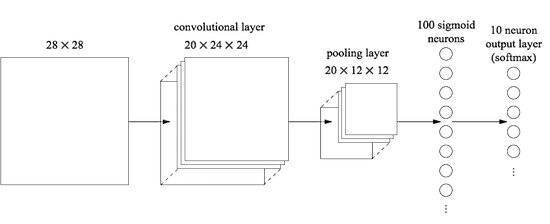
\includegraphics[width=0.917\textwidth]{images/simple_conv.png}
\end{center}

\noindent 在这个架构中，我们可以把卷积层和池化层看作是在学习输入训练图像的局部空间结构，而后面更靠后的全连接层则在更抽象的层次上学习，整合来自整个图像的全局信息. 这是卷积神经网络中一种常见的模式.

让我们训练这样一个网络，看看它的表现如何*\footnote{我在这里继续使用了小批量大小 $10$. 事实上，正如我们之前讨论的，使用更大的小批量可能可以加速训练. 我继续使用相同的小批量大小主要是为了与前面章节的实验保持一致.}:

\begin{lstlisting}
>>> net = Network([
        ConvPoolLayer(image_shape=(mini_batch_size, 1, 28, 28),
                      filter_shape=(20, 1, 5, 5),
                      poolsize=(2, 2)),
        FullyConnectedLayer(n_in=20*12*12, n_out=100),
        SoftmaxLayer(n_in=100, n_out=10)], mini_batch_size)
>>> net.SGD(training_data, 60, mini_batch_size, 0.1,
            validation_data, test_data)

\end{lstlisting}

这样我们就达到了 $98.78$ 百分比的准确率，这比我们之前任何结果都有了相当大的改进. 确实，我们把错误率降低了超过三分之一，这是一个很大的改进.

在指定网络结构时，我把卷积层和池化层当作一个单一的层. 它们是被视为单独的层还是单一的层，在某种程度上是个人偏好的问题. \texttt{network3.py} 把它们当作一个单一的层，因为这样可以使 \texttt{network3.py} 的代码更紧凑一些. 然而，如果需要的话，很容易修改 \texttt{network3.py} 使这些层可以被分别指定.

\begin{exerciseBox}{练习}

\begin{itemize}

\item 如果你省略全连接层，只使用卷积-池化层和 softmax 层，你会得到什么样的分类准确率？包含全连接层有帮助吗？

\end{itemize}

我们能否在 $98.78$ 百分比的分类准确率基础上进一步改进呢？

让我们尝试插入第二个卷积-池化层. 我们将把它插入到现有的卷积-池化层和全连接隐藏层之间. 同样，我们将使用 $5 \times 5$ 的局部感受野，并在 $2 \times 2$ 的区域上进行池化. 让我们看看使用与之前类似的超参数训练时会发生什么：

\begin{lstlisting}
>>> net = Network([
        ConvPoolLayer(image_shape=(mini_batch_size, 1, 28, 28),
                      filter_shape=(20, 1, 5, 5),
                      poolsize=(2, 2)),
        ConvPoolLayer(image_shape=(mini_batch_size, 20, 12, 12),
                      filter_shape=(40, 20, 5, 5),
                      poolsize=(2, 2)),
        FullyConnectedLayer(n_in=40*4*4, n_out=100),
        SoftmaxLayer(n_in=100, n_out=10)], mini_batch_size)
>>> net.SGD(training_data, 60, mini_batch_size, 0.1,
            validation_data, test_data)

\end{lstlisting}

又一次，我们得到了改进：我们现在达到了 $99.06$ 百分比的分类准确率！

在这一点上，有两个自然的问题要问. 第一个问题是：应用第二个卷积-池化层到底意味着什么？事实上，你可以把第二个卷积-池化层的输入看作是 $12 \times 12$ 的``图像''，其``像素''表示原始输入图像中特定局部化特征的存在（或缺失）. 所以你可以把这一层看作是以原始输入图像的一个版本作为输入. 那个版本是抽象化和浓缩过的，但仍然具有大量的空间结构，因此使用第二个卷积-池化层是有意义的.

这是一个令人满意的观点，但它引出了第二个问题. 前一层的输出涉及 $20$ 个独立的特征图，因此第二个卷积-池化层有 $20 \times 12 \times 12$ 个输入. 这就好像我们有 $20$ 个独立的图像输入到卷积-池化层，而不是像第一个卷积-池化层那样只有一个图像. 第二个卷积-池化层中的神经元应该如何响应这些多个输入图像呢？事实上，我们将允许这一层中的每个神经元从其局部感受野中的\emph{所有} $20 \times 5 \times 5$ 个输入神经元学习. 更非正式地说：第二个卷积-池化层中的特征检测器可以访问前一层的\emph{所有}特征，但仅限于它们特定的局部感受野内*\footnote{如果输入图像是彩色的，这个问题在第一个层中就会出现. 在那种情况下，每个像素会有 3 个输入特征，对应于输入图像中的红、绿、蓝通道. 所以我们会允许特征检测器访问所有颜色信息，但仅限于给定的局部感受野内.}.

\end{exerciseBox}

\begin{exerciseBox}{习题}

\begin{itemize}

\item \textbf{使用 tanh 激活函数} 在本书前面的几个地方，我提到过 tanh 函数可能是比 S 型函数更好的激活函数的论点. 我们从未按照那些建议去做，因为我们在使用 S 型函数时已经取得了足够的进展. 但现在让我们尝试一些使用 tanh 作为激活函数的实验. 尝试在卷积层和全连接层中使用 tanh 激活函数来训练网络*\footnote{注意你可以将 \texttt{activation\_\allowbreak{}fn=tanh} 作为参数传递给 \texttt{ConvPoolLayer} 和 \texttt{FullyConnectedLayer} 类.}. 从与 S 型网络相同的超参数开始，但训练 $20$ 个轮次而不是 $60$ 个. 你的网络表现如何？如果你继续训练到 $60$ 个轮次呢？尝试绘制基于 tanh 和基于 S 型的网络在每个轮次的验证准确率，一直到 $60$ 个轮次. 如果你的结果与我的相似，你会发现 tanh 网络训练得稍快一些，但最终准确率非常相似. 你能解释为什么 tanh 网络可能训练得更快吗？你能用 S 型函数获得类似的训练速度吗，也许通过改变学习率，或者做一些重新缩放*\footnote{你也许可以从回忆 $\sigma(z) = (1+\tanh(z/2))/2$ 中获得灵感.}？尝试对学习超参数或网络架构进行半打迭代，寻找 tanh 可能优于 S 型函数的方法. \emph{注意：这是一个开放性问题. 就我个人而言，我没有发现切换到 tanh 有多大优势，尽管我还没有进行详尽的实验，也许你可能会找到一种方法. 无论如何，稍后我们会发现切换到修正线性激活函数的优势，所以我们不会更深入地探讨 tanh 的使用.}

\end{itemize}

\textbf{使用修正线性单元：} 我们在这一点上开发的网络实际上是 1998 年那篇引入 MNIST 问题的开创性论文*\footnote{``Gradient-based learning applied to document recognition''，作者为 Yann LeCun, Léon Bottou, Yoshua Bengio，和 Patrick Haffner (1998). 在细节上有很多差异，但大致来说我们的网络与论文中描述的网络非常相似.}中使用的网络之一的一个变体，那个网络被称为 LeNet-5. 它是进一步实验以及建立理解和直觉的良好基础. 特别是，我们可以通过许多方式改变网络来尝试改进我们的结果.

作为一个开始，让我们改变我们的神经元，使其不使用 S 型激活函数，而是使用修正线性单元. 也就是说，我们将使用激活函数 $f(z) \equiv \max(0, z)$. 我们将训练 $60$ 个轮次，学习率为 $\eta = 0.03$. 我还发现使用一些 l2 正则化有一点帮助，正则化参数 $\lambda = 0.1$:

\begin{lstlisting}
>>> from network3 import ReLU
>>> net = Network([
        ConvPoolLayer(image_shape=(mini_batch_size, 1, 28, 28),
                      filter_shape=(20, 1, 5, 5),
                      poolsize=(2, 2),
                      activation_fn=ReLU),
        ConvPoolLayer(image_shape=(mini_batch_size, 20, 12, 12),
                      filter_shape=(40, 20, 5, 5),
                      poolsize=(2, 2),
                      activation_fn=ReLU),
        FullyConnectedLayer(n_in=40*4*4, n_out=100, activation_fn=ReLU),
        SoftmaxLayer(n_in=100, n_out=10)], mini_batch_size)
>>> net.SGD(training_data, 60, mini_batch_size, 0.03,
            validation_data, test_data, lmbda=0.1)

\end{lstlisting}

我获得了 $99.23$ 百分比的分类准确率. 这比 S 型函数的结果（$99.06$）有适度的改进. 然而，在我所有的实验中，我发现基于修正线性单元的网络始终优于基于 S 型激活函数的网络. 对于这个问题，转向修正线性单元似乎有真正的增益.

是什么使得修正线性激活函数比 S 型函数或 tanh 函数更好呢？目前，我们对这个问题的答案理解得很差. 确实，修正线性单元只是在过去几年才开始被广泛使用. 最近被采用的原因是经验性的：一些人尝试了修正线性单元，通常是基于直觉或启发式论证*\footnote{一个常见的理由是 $\max(0, z)$ 在 $z$ 很大时不会饱和，不像 S 型神经元，这有助于修正线性单元继续学习. 这个论证就其本身而言是好的，但它很难说是一个详细的论证，更像是一个想当然的故事. 注意我们在第 2 章讨论过饱和的问题.}. 他们在基准数据集分类上获得了好的结果，这种做法就传播开来了. 在一个理想的世界里，我们会有一个理论告诉我们对于哪种应用应该选择哪种激活函数. 但目前我们离这样的世界还很远. 如果通过更好的激活函数选择能够获得进一步的重大改进，我一点也不会感到惊讶. 我也期望在未来几十年里，一个强大的激活函数理论会被发展出来. 今天，我们仍然不得不依赖理解不足的经验法则和经验. \textbf{扩展训练数据：} 我们可能希望改进结果的另一种方法是通过算法扩展训练数据. 一种简单的扩展训练数据的方法是将每个训练图像平移一个像素，要么向上一个像素，向下一个像素，向左一个像素，或向右一个像素. 我们可以通过在 shell 提示符下运行程序 \texttt{expand\_\allowbreak{}mnist.py} 来做到这一点*\footnote{\texttt{expand\_\allowbreak{}mnist.py} 的代码可以在这里找到.}:

\begin{lstlisting}

$ python expand_mnist.py

\end{lstlisting}

运行这个程序会读取 $50,000$ 个 MNIST 训练图像，并准备一个扩展的训练集，包含 $250,000$ 个训练图像. 然后我们可以使用那些训练图像来训练我们的网络. 我们将使用与上面相同的网络，带有修正线性单元. 在我最初的实验中，我减少了训练轮次的数量——这是有道理的，因为我们用 $5$ 倍的数据进行训练. 但事实上，扩展数据结果大大减少了过拟合的影响. 因此，经过一些实验后，我最终回到了训练 $60$ 个轮次. 无论如何，让我们训练：

\begin{lstlisting}
>>> expanded_training_data, _, _ = network3.load_data_shared(
        "../data/mnist_expanded.pkl.gz")
>>> net = Network([
        ConvPoolLayer(image_shape=(mini_batch_size, 1, 28, 28),
                      filter_shape=(20, 1, 5, 5),
                      poolsize=(2, 2),
                      activation_fn=ReLU),
        ConvPoolLayer(image_shape=(mini_batch_size, 20, 12, 12),
                      filter_shape=(40, 20, 5, 5),
                      poolsize=(2, 2),
                      activation_fn=ReLU),
        FullyConnectedLayer(n_in=40*4*4, n_out=100, activation_fn=ReLU),
        SoftmaxLayer(n_in=100, n_out=10)], mini_batch_size)
>>> net.SGD(expanded_training_data, 60, mini_batch_size, 0.03,
            validation_data, test_data, lmbda=0.1)

\end{lstlisting}

使用扩展的训练数据，我获得了 $99.37$ 百分比的训练准确率. 所以这个几乎微不足道的变化带来了分类准确率的显著改进. 确实，正如我们之前讨论的，这种通过算法扩展数据的想法可以进一步推进. 只是为了提醒你之前讨论中一些结果的风味： 2003 年， Simard, Steinkraus 和 Platt*\footnote{Best Practices for Convolutional Neural Networks Applied to Visual Document Analysis，作者为 Patrice Simard, Dave Steinkraus，和 John Platt (2003).}使用一个在其他方面与我们的网络非常相似的神经网络，使用两个卷积-池化层，后面跟着一个包含 $100$ 个神经元的隐藏全连接层，将他们的 MNIST 性能提高到了 $99.6$ 百分比. 他们的架构在细节上有一些差异——例如，他们没有使用修正线性单元的优势——但他们改进性能的关键是扩展训练数据. 他们通过旋转、平移和倾斜 MNIST 训练图像来做到这一点. 他们还开发了一个``弹性扭曲''的过程，一种模拟人写字时手部肌肉经历的随机振荡的方法. 通过结合所有这些过程，他们大幅增加了训练数据的有效大小，这就是他们达到 $99.6$ 百分比准确率的方式.

\end{exerciseBox}
\begin{exerciseBox}{习题}

\begin{itemize}

\item 卷积层的理念是在图像上以不变的方式行事. 那么，当我们所做的只是平移输入数据时，我们的网络却能学到更多，这似乎令人惊讶. 你能解释为什么这实际上相当合理吗？

\end{itemize}

\textbf{插入一个额外的全连接层：} 我们能做得更好吗？一种可能是使用与上面完全相同的步骤，但扩大全连接层的规模. 我尝试了 $300$ 和 $1,000$ 个神经元，分别得到 $99.46$ 和 $99.43$ 百分比的结果. 这很有趣，但并不是对先前结果 ($99.37$ 百分比) 真正令人信服的超越.

那添加一个额外的全连接层呢？让我们尝试插入一个额外的全连接层，这样我们就有两个 $100$ 个隐藏神经元的全连接层：

\begin{lstlisting}
>>> net = Network([
        ConvPoolLayer(image_shape=(mini_batch_size, 1, 28, 28),
                      filter_shape=(20, 1, 5, 5),
                      poolsize=(2, 2),
                      activation_fn=ReLU),
        ConvPoolLayer(image_shape=(mini_batch_size, 20, 12, 12),
                      filter_shape=(40, 20, 5, 5),
                      poolsize=(2, 2),
                      activation_fn=ReLU),
        FullyConnectedLayer(n_in=40*4*4, n_out=100, activation_fn=ReLU),
        FullyConnectedLayer(n_in=100, n_out=100, activation_fn=ReLU),
        SoftmaxLayer(n_in=100, n_out=10)], mini_batch_size)
>>> net.SGD(expanded_training_data, 60, mini_batch_size, 0.03,
            validation_data, test_data, lmbda=0.1)

\end{lstlisting}

这样做，我得到了 $99.43$ 百分比的测试准确率. 同样，扩展后的网络并没有太大帮助. 用包含 $300$ 和 $1,000$ 个神经元的全连接层进行类似的实验，得到的结果分别为 $99.48$ 和 $99.47$ 百分比. 这令人鼓舞，但仍未达到真正决定性的超越.

这里发生了什么？是扩展的或额外的全连接层对 MNIST 真的没有帮助吗？还是我们的网络有能力做得更好，但我们学习的方式不对？例如，也许我们可以使用更强的正则化技术来减少过拟合的倾向. 一种可能是第 3 章介绍的 dropout 技术. 回想一下， dropout 的基本思想是在训练网络时随机移除单个激活值. 这使得模型对单个证据的丢失更加鲁棒，从而不太可能依赖于训练数据的特定特性. 让我们尝试将 dropout 应用于最后的全连接层：

\begin{lstlisting}
>>> net = Network([
        ConvPoolLayer(image_shape=(mini_batch_size, 1, 28, 28),
                      filter_shape=(20, 1, 5, 5),
                      poolsize=(2, 2),
                      activation_fn=ReLU),
        ConvPoolLayer(image_shape=(mini_batch_size, 20, 12, 12),
                      filter_shape=(40, 20, 5, 5),
                      poolsize=(2, 2),
                      activation_fn=ReLU),
        FullyConnectedLayer(
            n_in=40*4*4, n_out=1000, activation_fn=ReLU, p_dropout=0.5),
        FullyConnectedLayer(
            n_in=1000, n_out=1000, activation_fn=ReLU, p_dropout=0.5),
        SoftmaxLayer(n_in=1000, n_out=10, p_dropout=0.5)],
        mini_batch_size)
>>> net.SGD(expanded_training_data, 40, mini_batch_size, 0.03,
            validation_data, test_data)

\end{lstlisting}

使用这个，我们获得了 $99.60$ 百分比的准确率，这比我们之前的结果有了实质性的改进，尤其是我们的主要基准，即具有 $100$ 个隐藏神经元的网络，我们达到了 $99.37$ 百分比.

有两个变化值得注意.

首先，我将训练轮次减少到 $40$: dropout 减少了过拟合，因此我们学得更快.

其次，全连接隐藏层有 $1,000$ 个神经元，而不是之前使用的 $100$ 个. 当然， dropout 在训练时有效地省略了许多神经元，所以一些扩展是意料之中的. 事实上，我尝试了 $300$ 和 $1,000$ 个隐藏神经元的实验，并在 $1,000$ 个隐藏神经元上获得了 (非常轻微地) 更好的验证性能. \textbf{使用网络集成：} 进一步提高性能的一个简单方法是创建几个神经网络，然后让它们投票来确定最佳分类. 例如，假设我们使用上面的方案训练了 $5$ 个不同的神经网络，每个都达到了接近 $99.6$ 百分比的准确率. 即使这些网络都具有相似的准确率，由于不同的随机初始化，它们很可能会犯不同的错误. 在我们的 $5$ 个网络中进行投票可能会产生比任何单个网络更好的分类，这是合理的.

这听起来好得令人难以置信，但这种集成是神经网络和其他机器学习技术中常见的技巧. 它确实带来了进一步的改进：我们最终达到了 $99.67$ 百分比的准确率. 换句话说，我们的网络集成正确分类了 $10,000$ 张测试图像中除 $33$ 张之外的所有图像.

测试集中剩余的错误如下所示. 右上角的标签是根据 MNIST 数据的正确分类，而右下角是我们网络集成的输出标签：

\begin{center}
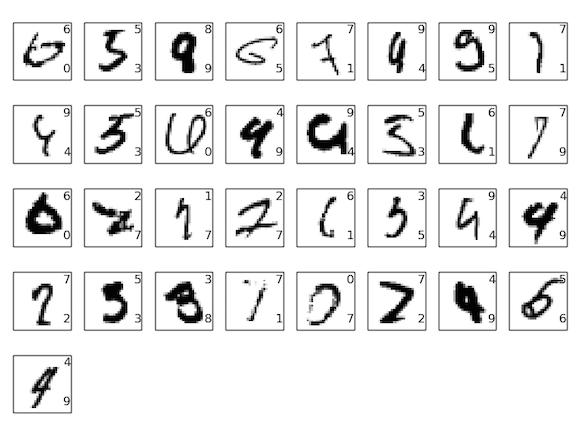
\includegraphics[width=0.967\textwidth]{images/ensemble_errors.png}
\end{center}

\noindent 值得详细查看这些. 前两个数字，一个 6 和一个 5，是我们集成的真实错误. 然而，它们也是可以理解的错误，是人类可能犯的那种错误. 那个 6 看起来确实很像 0，而 5 看起来很像 3. 第三张图像，据说是 8，实际上在我看来更像 9. 所以我在这里支持网络集成：我认为它比最初绘制数字的人做得更好. 另一方面，第四张图像，那个 6，确实似乎被我们的网络分类得很差.

以此类推. 在大多数情况下，我们网络的选择似乎至少是合理的，在某些情况下，它们在分类方面比最初写数字的人做得更好. 总的来说，我们的网络提供了卓越的性能，尤其是当你考虑到它们正确分类了未显示的 9,967 张图像时. 在这种背景下，这里少数明显的错误似乎相当可以理解. 即使是细心的人也会偶尔犯错. 因此，我预计只有极其细心和有条理的人才能做得更好. 我们的网络正在接近人类的表现. \textbf{为什么我们只对全连接层应用 dropout:} 如果你仔细查看上面的代码，你会注意到我们只对网络的全连接部分应用了 dropout，而不是卷积层. 原则上我们可以对卷积层应用类似的过程. 但实际上，没有必要：卷积层具有相当大的内置抗过拟合能力. 原因是共享权重意味着卷积滤波器被迫从整个图像中学习. 这使得它们不太可能捕捉到训练数据中的局部特性. 因此，不太需要应用其他正则化器，如 dropout. \textbf{更进一步：} 在 MNIST 上进一步提高性能是可能的. Rodrigo Benenson 编制了一个信息丰富的摘要页面，展示了多年来的进展，并附有论文链接. 这些论文中的许多都使用深度卷积网络，其思路与我们一直使用的网络类似. 如果你深入研究这些论文，你会发现许多有趣的技术，你可能会喜欢实现其中的一些. 如果你这样做，明智的做法是从一个可以快速训练的简单网络开始实现，这将帮助你更快地理解正在发生的事情.

在大多数情况下，我不会尝试综述这些最近的工作. 但我忍不住要做一个例外. 这是 Cireșan, Meier, Gambardella 和 Schmidhuber 在 2010 年的一篇论文*\footnote{Deep, Big, Simple Neural Nets Excel on Handwritten Digit Recognition, by Dan Claudiu Cireșan, Ueli Meier, Luca Maria Gambardella, and Jürgen Schmidhuber (2010).}. 我喜欢这篇论文的地方在于它多么简单. 该网络是一个多层神经网络，仅使用全连接层 (没有卷积). 他们最成功的网络隐藏层分别包含 $2,500$, $2,000$, $1,500$, $1,000$ 和 $500$ 个神经元. 他们使用类似于 Simard \emph{et al} 的想法来扩展他们的训练数据. 但除此之外，他们很少使用其他技巧，包括没有卷积层：这是一个普通的、香草味的网络，如果有足够的计算能力，只要有足够的耐心，在 1980 年代就可以训练出来 (如果 MNIST 数据集存在的话). 他们实现了 $99.65$ 百分比的分类准确率，或多或少与我们相同. 关键是使用一个非常大、非常深的网络，并使用 GPU 来加速训练. 这让他们能够训练许多轮次. 他们还利用他们长时间的训练逐渐将学习率从 $10^{-3}$ 降低到 $10^{-6}$. 尝试使用类似他们的架构来匹配这些结果是一个有趣的练习. \textbf{为什么我们能够训练？} 我们在上一章看到，在深层的多层神经网络中训练存在根本性的障碍. 特别是，我们看到梯度往往相当不稳定：当我们从输出层移动到较早的层时，梯度往往会消失 (梯度消失问题) 或爆炸 (梯度爆炸问题). 由于梯度是我们用来训练的信号，这会导致问题.

我们是如何避免这些结果的？

当然，答案是我们并没有避免这些结果. 相反，我们做了一些帮助我们无论如何都能继续的事情. 特别是： (1) 使用卷积层大大减少了这些层中的参数数量，使学习问题容易得多； (2) 使用更强大的正则化技术 (特别是 dropout 和卷积层) 来减少过拟合，这在更复杂的网络中否则是更大的问题； (3) 使用修正线性单元而不是 S 型神经元，以加速训练 - 根据经验，通常加快 $3$-$5$ 倍； (4) 使用 GPU 并愿意长时间训练. 特别是，在我们最后的实验中，我们使用比原始 MNIST 训练数据大 $5$ 倍的数据集训练了 $40$ 轮次. 在本书的早期，我们主要只使用原始训练数据训练 $30$ 轮次. 结合因素 (3) 和 (4)，就好像我们训练的时间比以前长了大约 $30$ 倍.

你的回答可能是 ``就这样吗？这就是我们训练深度网络所需要做的全部吗？有什么好大惊小怪的？''

当然，我们也使用了其他想法：利用足够大的数据集 (以帮助避免过拟合)；使用正确的代价函数 (以避免学习减慢)；使用良好的权重初始化 (也是为了避免学习减慢，由于神经元饱和)；通过算法扩展训练数据. 我们在前面的章节中讨论了这些和其他想法，并且在本章中大多能够在很少评论的情况下重用这些想法.

话虽如此，这确实是一组相当简单的想法. 简单，但协同使用时很强大. 开始深度学习已经变得相当容易了！ \textbf{这些网络到底有多深？} 将卷积-池化层计为单层，我们的最终架构有 $4$ 个隐藏层. 这样的网络真的配得上被称为\emph{深度}网络吗？当然， $4$ 个隐藏层比我们之前研究的浅层网络多得多. 那些网络大多只有一个隐藏层，或者偶尔有 $2$ 个隐藏层. 另一方面，截至 2015 年，最先进的深度网络有时有几十个隐藏层. 我偶尔听到人们采取比你更深的姿态，认为如果你在隐藏层数量上没有跟上潮流，那么你就不是真正在做深度学习. 我不认同这种态度，部分原因是它使深度学习的定义变成了依赖于当下结果的东西. 深度学习的真正突破是认识到超越在 2000 年代中期之前主导工作的浅层 $1$- 和 $2$-隐藏层网络是可行的. 这确实是一个重大的突破，开启了对更具表现力的模型的探索. 但除此之外，层数并不是主要的基本兴趣所在. 相反，使用更深的网络是一种工具，用于帮助实现其他目标 - 比如更好的分类准确率. \textbf{关于过程的一点说明：} 在本节中，我们已经顺利地从单隐藏层浅层网络过渡到多层卷积网络. 这一切看起来如此容易！我们做一个改变，并且在大多数情况下，我们得到了改进. 如果你开始实验，我可以保证事情不会总是那么顺利. 原因是我呈现了一个经过清理的叙述，省略了许多实验 - 包括许多失败的实验. 这个经过清理的叙述有望帮助你清楚地了解基本想法. 但它也有传达不完整印象的风险. 获得一个好的、可工作的网络可能涉及大量的试错，以及偶尔的挫折. 在实践中，你应该预期会进行相当多的实验. 为了加快这个过程，你可能会发现重新审视第 3 章关于如何选择神经网络超参数的讨论很有帮助，也许还可以看看该节中建议的一些进一步阅读.

\end{exerciseBox}
\sectionTitle{卷积网络的代码}{卷积网络的代码}

好的，让我们来看看我们程序的代码，\texttt{network3.py}. 在结构上，它类似于我们在第 3 章开发的程序 \texttt{network2.py}，尽管由于使用了 Theano，细节有所不同. 我们将从 \texttt{FullyConnectedLayer} 类开始看起，它类似于本书前面研究过的层. 代码如下（讨论见后）*\footnote{2016 年 11 月注：几位读者指出，在初始化 \texttt{self.w} 的那一行，我设置了 \texttt{scale=np.sqrt(1.0/n\_\allowbreak{}out)}，而第 3 章的论证表明更好的初始化可能是 \texttt{scale=np.sqrt(1.0/n\_\allowbreak{}in)}. 这纯粹是我的一个错误. 在理想情况下，我会用正确的代码重新运行本章的所有示例. 不过，我已经转向了其他项目，所以就让这个错误保留吧.}：

\begin{lstlisting}
class FullyConnectedLayer(object):

    def __init__(self, n_in, n_out, activation_fn=sigmoid, p_dropout=0.0):
        self.n_in = n_in
        self.n_out = n_out
        self.activation_fn = activation_fn
        self.p_dropout = p_dropout
        # Initialize weights and biases
        self.w = theano.shared(
            np.asarray(
                np.random.normal(
                    loc=0.0, scale=np.sqrt(1.0/n_out), size=(n_in, n_out)),
                dtype=theano.config.floatX),
            name='w', borrow=True)
        self.b = theano.shared(
            np.asarray(np.random.normal(loc=0.0, scale=1.0, size=(n_out,)),
                       dtype=theano.config.floatX),
            name='b', borrow=True)
        self.params = [self.w, self.b]

    def set_inpt(self, inpt, inpt_dropout, mini_batch_size):
        self.inpt = inpt.reshape((mini_batch_size, self.n_in))
        self.output = self.activation_fn(
            (1-self.p_dropout)*T.dot(self.inpt, self.w) + self.b)
        self.y_out = T.argmax(self.output, axis=1)
        self.inpt_dropout = dropout_layer(
            inpt_dropout.reshape((mini_batch_size, self.n_in)), self.p_dropout)
        self.output_dropout = self.activation_fn(
            T.dot(self.inpt_dropout, self.w) + self.b)

    def accuracy(self, y):
        "Return the accuracy for the mini-batch."
        return T.mean(T.eq(y, self.y_out))

\end{lstlisting}

\texttt{\_\allowbreak{}\_\allowbreak{}init\_\allowbreak{}\_\allowbreak{}} 方法的大部分内容不言自明，但有几句话可能有助于阐明代码. 按照惯例，我们将权重和偏置随机初始化为具有适当标准差的正态随机变量. 执行此操作的代码行看起来有点吓人. 然而，大部分复杂性只是将权重和偏置加载到 Theano 所称的共享变量中. 这确保了这些变量可以在 GPU 上处理，如果有可用的 GPU 的话. 我们不会过多深入细节. 如果你感兴趣，可以深入研究 Theano 文档. 另请注意，这种权重和偏置初始化是为 S 型激活函数设计的（如前所述）. 理想情况下，对于 tanh 和修正线性函数等激活函数，我们会以略有不同的方式初始化权重和偏置. 这将在下面的习题中进一步讨论.\texttt{\_\allowbreak{}\_\allowbreak{}init\_\allowbreak{}\_\allowbreak{}} 方法以 \texttt{self.params = [self.w, self.b]} 结束. 这是一种便捷的方式，用于捆绑与该层相关的所有可学习参数. 稍后，\texttt{Network.SGD} 方法将使用 \texttt{params} 属性来确定 \texttt{Network} 实例中哪些变量可以学习.

\texttt{set\_\allowbreak{}inpt} 方法用于设置层的输入，并计算相应的输出. 我使用名称 \texttt{inpt} 而不是 \texttt{input}，因为 \texttt{input} 是 Python 的内置函数，而干扰内置函数往往会导致不可预测的行为和难以诊断的错误. 请注意，我们实际上以两种不同的方式设置输入：作为 \texttt{self.inpt} 和 \texttt{self.inpt\_\allowbreak{}dropout}. 这样做是因为在训练期间我们可能想要使用 dropout. 如果是这种情况，那么我们希望移除比例为 \texttt{self.p\_\allowbreak{}dropout} 的神经元. 这就是 \texttt{set\_\allowbreak{}inpt} 方法倒数第二行中的函数 \texttt{dropout\_\allowbreak{}layer} 所做的. 因此，\texttt{self.inpt\_\allowbreak{}dropout} 和 \texttt{self.output\_\allowbreak{}dropout} 在训练期间使用，而 \texttt{self.inpt} 和 \texttt{self.output} 用于所有其他目的，例如，评估验证数据和测试数据上的准确率.

\texttt{ConvPoolLayer} 和 \texttt{SoftmaxLayer} 类的定义与 \texttt{FullyConnectedLayer} 类似. 事实上，它们如此接近，以至于我不会在这里摘录代码. 如果你感兴趣，可以查看本节后面 \texttt{network3.py} 的完整列表.

然而，一些细节上的微小差异值得一提. 最明显的是，在 \texttt{ConvPoolLayer} 和 \texttt{SoftmaxLayer} 中，我们以适合该层类型的方式计算输出激活值. 幸运的是，Theano 使这变得容易，提供了内置操作来计算卷积、最大池化和 softmax 函数.

不太明显的是，当我们引入 softmax 层时，我们从未讨论过如何初始化权重和偏置. 在其他地方，我们论证过对于 S 型层，我们应该使用适当参数化的正态随机变量来初始化权重. 但那个启发式论证是特定于 S 型神经元的（并且，经过一些修正，也适用于 tanh 神经元）. 然而，没有特别的理由认为该论证应该适用于 softmax 层. 因此，没有\emph{先验}理由再次应用该初始化. 与其这样做，我将所有

好的，我们已经看过了所有的层类. 那么 \texttt{Network} 类呢？让我们从 \texttt{\_\allowbreak{}\_\allowbreak{}init\_\allowbreak{}\_\allowbreak{}} 方法开始看起：

\begin{lstlisting}
class Network(object):

    def __init__(self, layers, mini_batch_size):
        """Takes a list of `layers`, describing the network architecture, and
        a value for the `mini_batch_size` to be used during training
        by stochastic gradient descent.

        """
        self.layers = layers
        self.mini_batch_size = mini_batch_size
        self.params = [param for layer in self.layers for param in layer.params]
        self.x = T.matrix("x")
        self.y = T.ivector("y")
        init_layer = self.layers[0]
        init_layer.set_inpt(self.x, self.x, self.mini_batch_size)
        for j in xrange(1, len(self.layers)):
            prev_layer, layer  = self.layers[j-1], self.layers[j]
            layer.set_inpt(
                prev_layer.output, prev_layer.output_dropout, self.mini_batch_size)
        self.output = self.layers[-1].output
        self.output_dropout = self.layers[-1].output_dropout

\end{lstlisting}

这里的大部分内容不言自明，或者几乎如此.\texttt{self.params = [param for layer in...]} 这一行将每一层的参数捆绑到一个列表中. 正如上面所预期的，\texttt{Network.SGD} 方法将使用 \texttt{self.params} 来确定 \texttt{Network} 中哪些变量可以学习.\texttt{self.x = T.matrix(``x'')} 和 \texttt{self.y = T.ivector(``y'')} 这两行定义了名为 \texttt{x} 和 \texttt{y} 的 Theano 符号变量. 这些将用于表示网络的输入和期望输出.

现在，这不是一篇 Theano 教程，因此我们不会过于深入地探讨这些符号变量意味着什么*\footnote{Theano 文档提供了对 Theano 的良好介绍. 如果你遇到困难，查看网上其他可用的教程之一可能会有所帮助. 例如，本教程涵盖了许多基础知识.}. 但大致的想法是，它们代表数学变量，\emph{而非}显式的值. 我们可以对这些变量做所有通常可以做的事情：加、减、乘它们，应用函数，等等. 事实上，Theano 提供了许多操作这类符号变量的方法，比如做卷积、最大池化等等. 但最大的优势是能够使用一种非常通用的反向传播算法形式来进行快速的符号微分. 这对于将随机梯度下降应用于各种各样的网络架构极为有用. 特别是，接下来的几行代码定义了网络的符号输出. 我们首先设置初始层的输入，代码如下：

\begin{lstlisting}
        init_layer.set_inpt(self.x, self.x, self.mini_batch_size)

\end{lstlisting}

请注意，输入是一次一个小批量设置的，这就是小批量大小存在的原因. 另请注意，我们将输入 \texttt{self.x} 传递了两次：这是因为我们可能以两种不同的方式使用网络（使用或不使用 dropout）. 然后 \texttt{for} 循环将符号变量 \texttt{self.x} 向前传播通过 \texttt{Network} 的各层. 这允许我们定义最终的 \texttt{output} 和 \texttt{output\_\allowbreak{}dropout} 属性，它们符号化地表示 \texttt{Network} 的输出.

现在我们已经理解了 \texttt{Network} 是如何初始化的，让我们看看它是如何训练的，即使用 \texttt{SGD} 方法. 代码看起来很长，但其结构实际上相当简单. 代码后面有解释性注释.

\begin{lstlisting}
    def SGD(self, training_data, epochs, mini_batch_size, eta,
            validation_data, test_data, lmbda=0.0):
        """Train the network using mini-batch stochastic gradient descent."""
        training_x, training_y = training_data
        validation_x, validation_y = validation_data
        test_x, test_y = test_data

        # compute number of minibatches for training, validation and testing
        num_training_batches = size(training_data)/mini_batch_size
        num_validation_batches = size(validation_data)/mini_batch_size
        num_test_batches = size(test_data)/mini_batch_size

        # define the (regularized) cost function, symbolic gradients, and updates
        l2_norm_squared = sum([(layer.w**2).sum() for layer in self.layers])
        cost = self.layers[-1].cost(self)+\
               0.5*lmbda*l2_norm_squared/num_training_batches
        grads = T.grad(cost, self.params)
        updates = [(param, param-eta*grad)
                   for param, grad in zip(self.params, grads)]

        # define functions to train a mini-batch, and to compute the
        # accuracy in validation and test mini-batches.
        i = T.lscalar() # mini-batch index
        train_mb = theano.function(
            [i], cost, updates=updates,
            givens={
                self.x:
                training_x[i*self.mini_batch_size: (i+1)*self.mini_batch_size],
                self.y:
                training_y[i*self.mini_batch_size: (i+1)*self.mini_batch_size]
            })
        validate_mb_accuracy = theano.function(
            [i], self.layers[-1].accuracy(self.y),
            givens={
                self.x:
                validation_x[i*self.mini_batch_size: (i+1)*self.mini_batch_size],
                self.y:
                validation_y[i*self.mini_batch_size: (i+1)*self.mini_batch_size]
            })
        test_mb_accuracy = theano.function(
            [i], self.layers[-1].accuracy(self.y),
            givens={
                self.x:
                test_x[i*self.mini_batch_size: (i+1)*self.mini_batch_size],
                self.y:
                test_y[i*self.mini_batch_size: (i+1)*self.mini_batch_size]
            })
        self.test_mb_predictions = theano.function(
            [i], self.layers[-1].y_out,
            givens={
                self.x:
                test_x[i*self.mini_batch_size: (i+1)*self.mini_batch_size]
            })
        # Do the actual training
        best_validation_accuracy = 0.0
        for epoch in xrange(epochs):
            for minibatch_index in xrange(num_training_batches):
                iteration = num_training_batches*epoch+minibatch_index
                if iteration
                    print("Training mini-batch number {0}".format(iteration))
                cost_ij = train_mb(minibatch_index)
                if (iteration+1)
                    validation_accuracy = np.mean(
                        [validate_mb_accuracy(j) for j in xrange(num_validation_batches)])
                    print("Epoch {0}: validation accuracy {1:.2
                        epoch, validation_accuracy))
                    if validation_accuracy >= best_validation_accuracy:
                        print("This is the best validation accuracy to date.")
                        best_validation_accuracy = validation_accuracy
                        best_iteration = iteration
                        if test_data:
                            test_accuracy = np.mean(
                                [test_mb_accuracy(j) for j in xrange(num_test_batches)])
                            print('The corresponding test accuracy is {0:.2
                                test_accuracy))
        print("Finished training network.")
        print("Best validation accuracy of {0:.2
            best_validation_accuracy, best_iteration))
        print("Corresponding test accuracy of {0:.2

\end{lstlisting}

前几行很直接，将数据集分为 $x$ 和 $y$ 分量，并计算每个数据集中使用的小批量的数量. 接下来的几行更有趣，展示了 Theano 使用起来有趣的一些方面. 让我们在这里明确摘录这些行：
\begin{lstlisting}
        # define the (regularized) cost function, symbolic gradients, and updates
        l2_norm_squared = sum([(layer.w**2).sum() for layer in self.layers])
        cost = self.layers[-1].cost(self)+\
               0.5*lmbda*l2_norm_squared/num_training_batches
        grads = T.grad(cost, self.params)
        updates = [(param, param-eta*grad)
                   for param, grad in zip(self.params, grads)]

\end{lstlisting}

在这些代码行中，我们以符号方式建立了正则化的对数似然代价函数，在梯度函数中计算相应的导数，以及相应的参数更新.Theano 让我们仅用这几行代码就实现了所有这些. 唯一隐藏的是，计算 \texttt{cost} 涉及对输出层的 \texttt{cost} 方法的调用；那段代码在 \texttt{network3.py} 的其他地方. 但那段代码无论如何都很简短. 定义了所有这些之后，就可以定义 \texttt{train\_\allowbreak{}mb} 函数了，这是一个 Theano 符号函数，它使用 \texttt{updates} 来更新 \texttt{Network} 参数，给定一个小批量索引. 类似地，\texttt{validate\_\allowbreak{}mb\_\allowbreak{}accuracy} 和 \texttt{test\_\allowbreak{}mb\_\allowbreak{}accuracy} 计算 \texttt{Network} 在任何给定的验证或测试数据小批量上的准确率. 通过对这些函数取平均，我们将能够计算整个验证和测试数据集上的准确率.

\texttt{SGD} 方法的其余部分不言自明——我们只是遍历轮次，反复在小批量训练数据上训练网络，并计算验证和测试准确率.

好了，我们现在已经理解了 \texttt{network3.py} 中最重要的代码片段. 让我们简要地看一下整个程序. 你不需要详细阅读它，但你可能喜欢浏览一下，也许深入到你感兴趣的任何部分. 真正理解它的最好方法当然是修改它、添加额外功能，或者重构任何你认为可以做得更优雅的地方. 代码之后有一些习题，其中包含一些入门的建议. 以下是代码*\footnote{在 GPU 上使用 Theano 可能有点棘手. 特别是，很容易犯从 GPU 上拉取数据的错误，这会大大降低速度. 我试图避免这一点. 话虽如此，通过仔细优化 Theano 的配置，这段代码肯定还可以进一步加速不少. 更多细节请参阅 Theano 文档.}：

\begin{lstlisting}
"""network3.py
~~~~~~~~~~~~~~

A Theano-based program for training and running simple neural
networks.

Supports several layer types (fully connected, convolutional, max
pooling, softmax), and activation functions (sigmoid, tanh, and
rectified linear units, with more easily added).

When run on a CPU, this program is much faster than network.py and
network2.py.  However, unlike network.py and network2.py it can also
be run on a GPU, which makes it faster still.

Because the code is based on Theano, the code is different in many
ways from network.py and network2.py.  However, where possible I have
tried to maintain consistency with the earlier programs.  In
particular, the API is similar to network2.py.  Note that I have
focused on making the code simple, easily readable, and easily
modifiable.  It is not optimized, and omits many desirable features.

This program incorporates ideas from the Theano documentation on
convolutional neural nets (notably,
http://deeplearning.net/tutorial/lenet.html ), from Misha Denil's
implementation of dropout (https://github.com/mdenil/dropout ), and
from Chris Olah (http://colah.github.io ).

Written for Theano 0.6 and 0.7, needs some changes for more recent
versions of Theano.

"""

#### Libraries
# Standard library
import cPickle
import gzip

# Third-party libraries
import numpy as np
import theano
import theano.tensor as T
from theano.tensor.nnet import conv
from theano.tensor.nnet import softmax
from theano.tensor import shared_randomstreams
from theano.tensor.signal import downsample

# Activation functions for neurons
def linear(z): return z
def ReLU(z): return T.maximum(0.0, z)
from theano.tensor.nnet import sigmoid
from theano.tensor import tanh

#### Constants
GPU = True
if GPU:
    print "Trying to run under a GPU.  If this is not desired, then modify "+\
        "network3.py\nto set the GPU flag to False."
    try: theano.config.device = 'gpu'
    except: pass # it's already set
    theano.config.floatX = 'float32'
else:
    print "Running with a CPU.  If this is not desired, then the modify "+\
        "network3.py to set\nthe GPU flag to True."

#### Load the MNIST data
def load_data_shared(filename="../data/mnist.pkl.gz"):
    f = gzip.open(filename, 'rb')
    training_data, validation_data, test_data = cPickle.load(f)
    f.close()
    def shared(data):
        """Place the data into shared variables.  This allows Theano to copy
        the data to the GPU, if one is available.

        """
        shared_x = theano.shared(
            np.asarray(data[0], dtype=theano.config.floatX), borrow=True)
        shared_y = theano.shared(
            np.asarray(data[1], dtype=theano.config.floatX), borrow=True)
        return shared_x, T.cast(shared_y, "int32")
    return [shared(training_data), shared(validation_data), shared(test_data)]

#### Main class used to construct and train networks
class Network(object):

    def __init__(self, layers, mini_batch_size):
        """Takes a list of `layers`, describing the network architecture, and
        a value for the `mini_batch_size` to be used during training
        by stochastic gradient descent.

        """
        self.layers = layers
        self.mini_batch_size = mini_batch_size
        self.params = [param for layer in self.layers for param in layer.params]
        self.x = T.matrix("x")
        self.y = T.ivector("y")
        init_layer = self.layers[0]
        init_layer.set_inpt(self.x, self.x, self.mini_batch_size)
        for j in xrange(1, len(self.layers)):
            prev_layer, layer  = self.layers[j-1], self.layers[j]
            layer.set_inpt(
                prev_layer.output, prev_layer.output_dropout, self.mini_batch_size)
        self.output = self.layers[-1].output
        self.output_dropout = self.layers[-1].output_dropout

    def SGD(self, training_data, epochs, mini_batch_size, eta,
            validation_data, test_data, lmbda=0.0):
        """Train the network using mini-batch stochastic gradient descent."""
        training_x, training_y = training_data
        validation_x, validation_y = validation_data
        test_x, test_y = test_data

        # compute number of minibatches for training, validation and testing
        num_training_batches = size(training_data)/mini_batch_size
        num_validation_batches = size(validation_data)/mini_batch_size
        num_test_batches = size(test_data)/mini_batch_size

        # define the (regularized) cost function, symbolic gradients, and updates
        l2_norm_squared = sum([(layer.w**2).sum() for layer in self.layers])
        cost = self.layers[-1].cost(self)+\
               0.5*lmbda*l2_norm_squared/num_training_batches
        grads = T.grad(cost, self.params)
        updates = [(param, param-eta*grad)
                   for param, grad in zip(self.params, grads)]

        # define functions to train a mini-batch, and to compute the
        # accuracy in validation and test mini-batches.
        i = T.lscalar() # mini-batch index
        train_mb = theano.function(
            [i], cost, updates=updates,
            givens={
                self.x:
                training_x[i*self.mini_batch_size: (i+1)*self.mini_batch_size],
                self.y:
                training_y[i*self.mini_batch_size: (i+1)*self.mini_batch_size]
            })
        validate_mb_accuracy = theano.function(
            [i], self.layers[-1].accuracy(self.y),
            givens={
                self.x:
                validation_x[i*self.mini_batch_size: (i+1)*self.mini_batch_size],
                self.y:
                validation_y[i*self.mini_batch_size: (i+1)*self.mini_batch_size]
            })
        test_mb_accuracy = theano.function(
            [i], self.layers[-1].accuracy(self.y),
            givens={
                self.x:
                test_x[i*self.mini_batch_size: (i+1)*self.mini_batch_size],
                self.y:
                test_y[i*self.mini_batch_size: (i+1)*self.mini_batch_size]
            })
        self.test_mb_predictions = theano.function(
            [i], self.layers[-1].y_out,
            givens={
                self.x:
                test_x[i*self.mini_batch_size: (i+1)*self.mini_batch_size]
            })
        # Do the actual training
        best_validation_accuracy = 0.0
        for epoch in xrange(epochs):
            for minibatch_index in xrange(num_training_batches):
                iteration = num_training_batches*epoch+minibatch_index
                if iteration
                    print("Training mini-batch number {0}".format(iteration))
                cost_ij = train_mb(minibatch_index)
                if (iteration+1)
                    validation_accuracy = np.mean(
                        [validate_mb_accuracy(j) for j in xrange(num_validation_batches)])
                    print("Epoch {0}: validation accuracy {1:.2
                        epoch, validation_accuracy))
                    if validation_accuracy >= best_validation_accuracy:
                        print("This is the best validation accuracy to date.")
                        best_validation_accuracy = validation_accuracy
                        best_iteration = iteration
                        if test_data:
                            test_accuracy = np.mean(
                                [test_mb_accuracy(j) for j in xrange(num_test_batches)])
                            print('The corresponding test accuracy is {0:.2
                                test_accuracy))
        print("Finished training network.")
        print("Best validation accuracy of {0:.2
            best_validation_accuracy, best_iteration))
        print("Corresponding test accuracy of {0:.2

#### Define layer types

class ConvPoolLayer(
\end{lstlisting}
